In this section a basic idea of how the user interface should look like when shown. It presents the basic login and signup tabs, the main tab showing the usable services, and a specific tab for each distinct service. The mockups are very similar for different kinds of users, only the services provided differ. For instance, \ref{mainTab1} provide the services that only the citizens can use, whereas \ref{mainTab2} shows the additional services that the authorities and municipality users can use.

\subsubsection{Mobile app common interfaces}

\begin{figure}[H]
	\centering
	\begin{minipage}[b]{0.38\linewidth}
		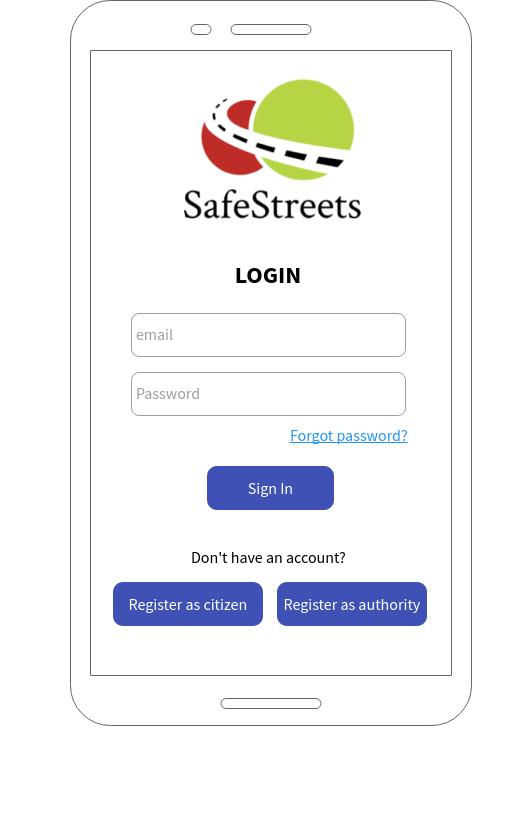
\includegraphics[width=\linewidth]{Mock/LoginMock}
	    \caption{Login tab.}
	\end{minipage}
	\begin{minipage}[b]{0.38\linewidth}
	    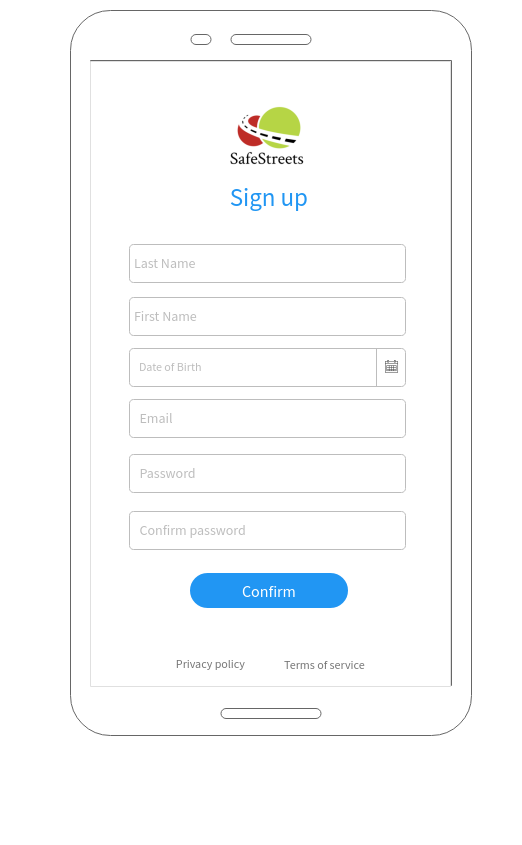
\includegraphics[width=\linewidth]{Mock/SignupMock}
	    \caption{Signup tab.}
	\end{minipage}
\end{figure}

\begin{figure}[H]
	\centering
		\begin{minipage}[b]{0.38\linewidth}
		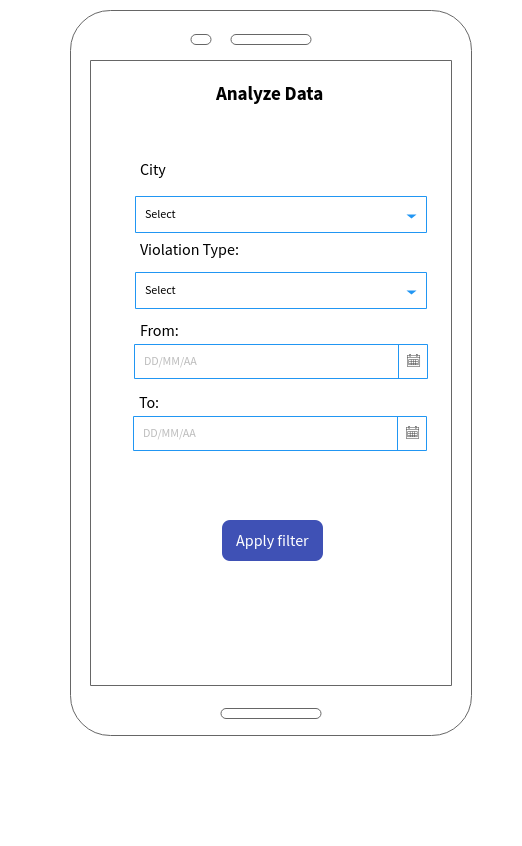
\includegraphics[width=\linewidth]{Mock/AnalyzeDataMock}
		\caption{Analyze data.}
	\end{minipage}
	\begin{minipage}[b]{0.38\linewidth}
		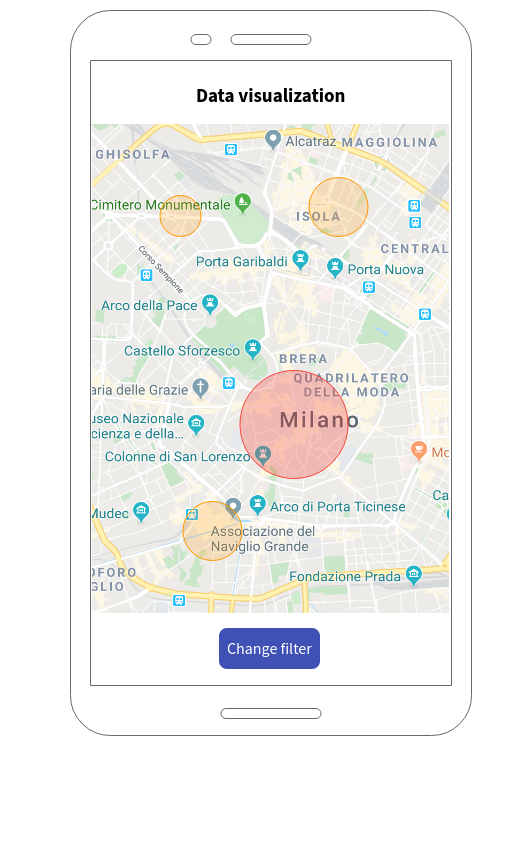
\includegraphics[width=\linewidth]{Mock/DataVisualizationMock}
		\caption{Data visualization.}
	\end{minipage}
\end{figure}

\subsubsection{Citizen interfaces}

\begin{figure}[H]
	\centering
		\begin{minipage}[b]{0.328\linewidth}
		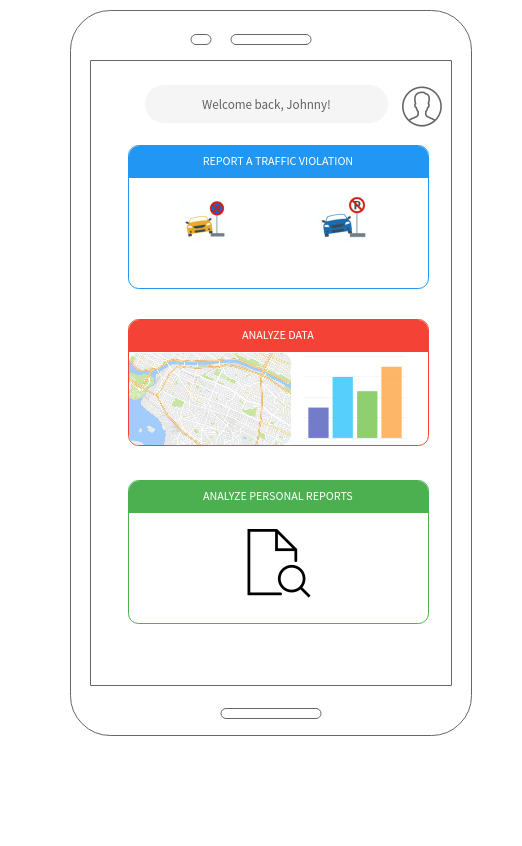
\includegraphics[width=\linewidth]{Mock/MainTabMock1}
		\caption{Main tab 1.}
		\label{mainTab1}
	\end{minipage}
	\begin{minipage}[b]{0.328\linewidth}
		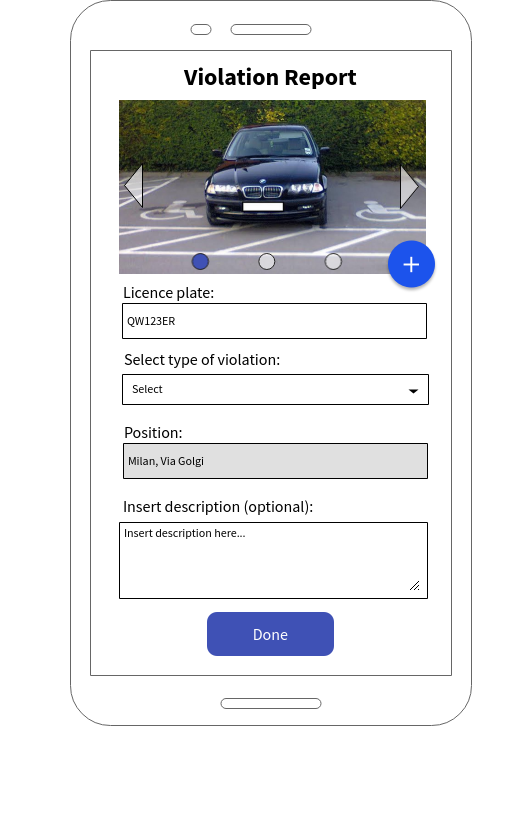
\includegraphics[width=\linewidth]{Mock/ReportMock}
		\caption{Report tab.}
	\end{minipage}
	\begin{minipage}[b]{0.328\linewidth}
		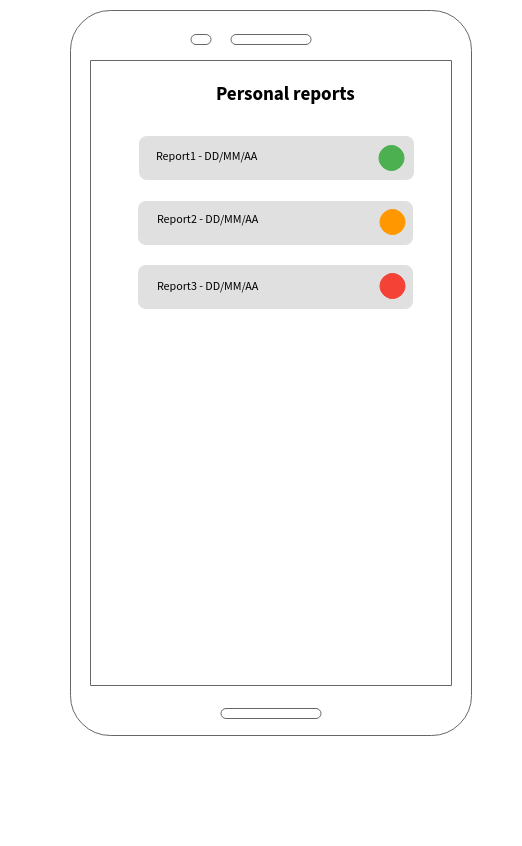
\includegraphics[width=\linewidth]{Mock/PersonalReportsMock}
		\caption{Done reports.}
	\end{minipage}	
\end{figure}

\begin{figure}[H]
	\centering
	\begin{minipage}[b]{0.99\linewidth}
		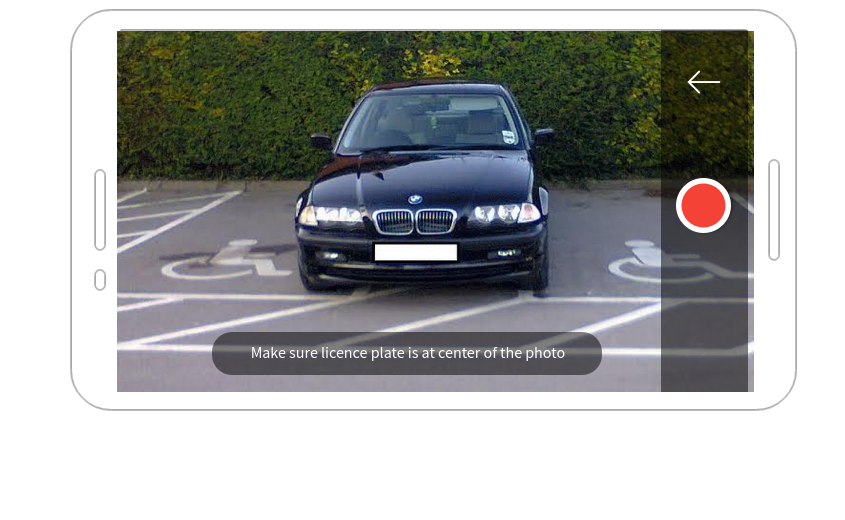
\includegraphics[width=\linewidth]{Mock/PhotoMock}
		\caption{Violation photo.}
	\end{minipage}
\end{figure}

\subsubsection{Authorities interfaces}

\begin{figure}[H]
	\centering
	\begin{minipage}[b]{0.4\linewidth}
		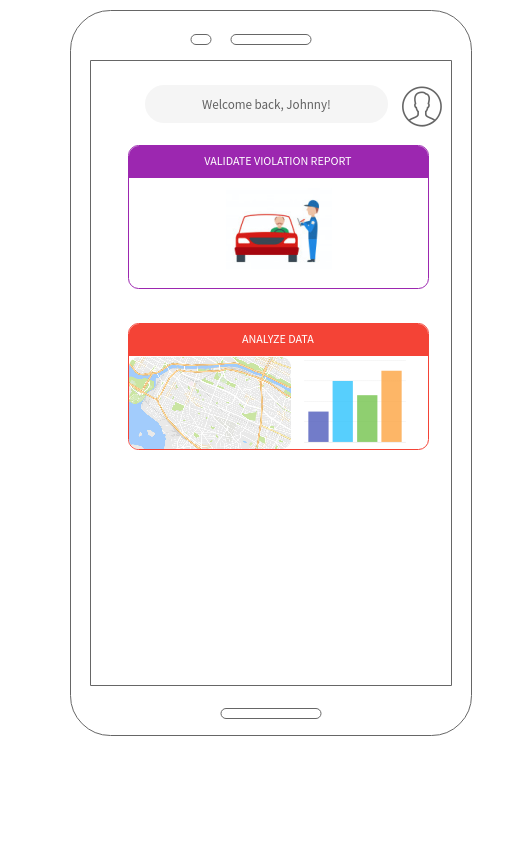
\includegraphics[width=\linewidth]{Mock/MainTabMock2}
		\caption{Main tab 2.}
		\label{mainTab2}
	\end{minipage}
	\begin{minipage}[b]{0.4\linewidth}
		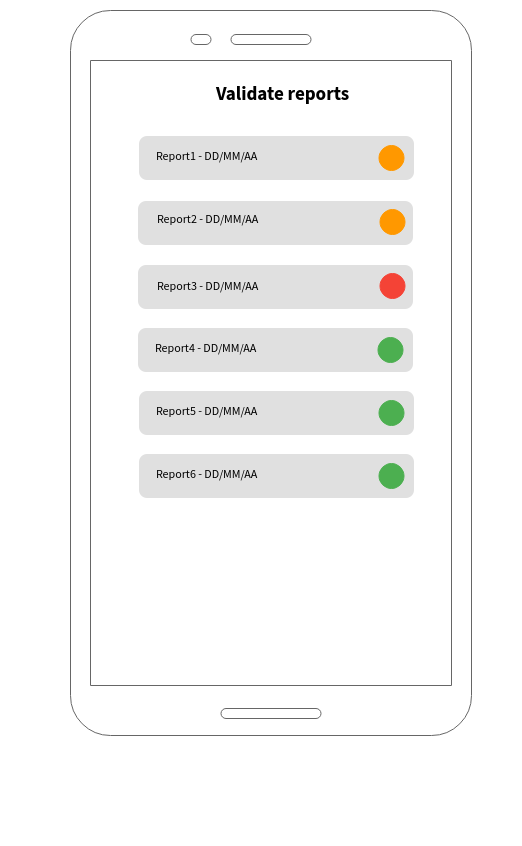
\includegraphics[width=\linewidth]{Mock/ValidateReportsMock}
		\caption{Validate reports.}
	\end{minipage}
\end{figure}

\subsubsection{Municipality interfaces}

\begin{figure}[H]
	\centering
	\begin{minipage}[b]{0.4\linewidth}
	    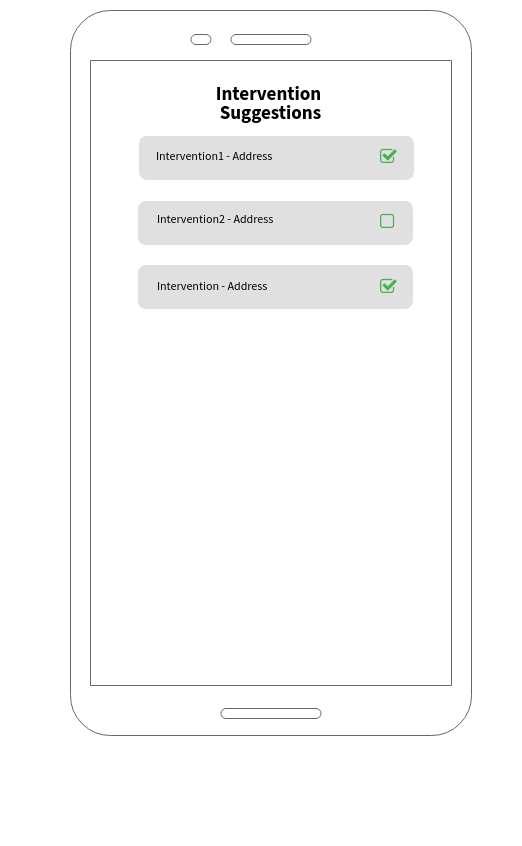
\includegraphics[width=\linewidth]{Mock/InterventionMock}
	    \caption{Interventions.}
	\end{minipage}
\end{figure}




